%! Rational Functions and Zeros — Unit 1, Lesson 1.8 — Group Activity
\documentclass[10pt]{article}
\usepackage{precalculus-article}
\usepackage{precalculus-boxes}
\newcommand{\TallMath}[1]{$\displaystyle #1\rule[-1.4em]{0pt}{3.2em}$}

\begin{document}

\pageheader{Unit 1, Lesson 1.8}{Group Activity}
\namepartnerperiod

\vspace{0.10in}

\begin{scenariobox}[Break-Even Analysis]{sky}
\small
A factory models its profit (or loss) per unit using the rational function
\[
  r(x) = \frac{x^2 - 7x + 10}{x - 4},
\]
where $x > 0$ represents units produced (in hundreds) and $x \ne 4$.
Positive values of $r(x)$ mean profit; negative values mean loss.
\end{scenariobox}

\vspace{0.08in}

\begin{tcolorbox}[colback=white, colframe=black!40,
    title=\textbf{Tier R --- Remediate},
    fonttitle=\bfseries, arc=2mm, left=3mm, right=3mm, top=2mm, bottom=2mm]

\begin{enumerate}[itemsep=10pt]

  \item Factor the numerator $x^2 - 7x + 10$ completely.

        $x^2 - 7x + 10 = $ \blank{6cm}

  \item At what values of $x$ does $r(x) = 0$? (Set the factored numerator equal to zero.)

        $x = $ \blank{5cm}

  \item Is $x = 4$ in the domain of $r$? \quad \textbf{Yes} \quad / \quad \textbf{No} \quad
        (Circle one.)

        Why? \blank{8cm}

  \item List ALL critical values (zeros of numerator AND zeros of denominator) below on the number line.
        Mark numerator zeros with a closed dot ($\bullet$) and the denominator zero with an open dot ($\circ$).

        \vspace{0.18in}
        \begin{center}
        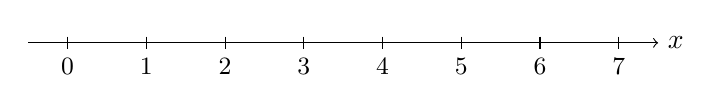
\begin{tikzpicture}
          \draw[->] (-0.5,0) -- (7.5,0) node[right] {$x$};
          \foreach \x in {0,1,2,3,4,5,6,7} {
            \draw (\x,0.08) -- (\x,-0.08) node[below] {\small\x};
          }
        \end{tikzpicture}
        \end{center}
\end{enumerate}
\end{tcolorbox}

\vspace{0.08in}

\begin{tcolorbox}[colback=white, colframe=black!40,
    title=\textbf{Tier A --- Apply},
    fonttitle=\bfseries, arc=2mm, left=3mm, right=3mm, top=2mm, bottom=2mm]

\begin{enumerate}[itemsep=10pt]

  \item Find all zeros of $r(x) = \dfrac{x^2 - 7x + 10}{x - 4}$.
        Show your steps (find domain restriction, factor numerator, check domain).

        \vspace{0.08in}
        Domain restriction: \blank{3cm} \qquad
        Numerator zeros: \blank{3.5cm} \qquad
        Zeros of $r$: \blank{3cm}

  \item Complete the sign chart below for $r(x)$.

        \medskip
        \begin{center}
        \renewcommand{\arraystretch}{1.6}
        \begin{tabular}{|c|c|c|c|c|}
        \hline
        \textbf{Interval} & $(0,\,2)$ & $(2,\,4)$ & $(4,\,5)$ & $(5,\,\infty)$ \\
        \hline
        Test value  & \blank{1.5cm} & \blank{1.5cm} & \blank{1.5cm} & \blank{1.5cm} \\
        \hline
        Sign of $r$ & \blank{1.5cm} & \blank{1.5cm} & \blank{1.5cm} & \blank{1.5cm} \\
        \hline
        \end{tabular}
        \end{center}

  \item Solve $r(x) \geq 0$ (units where profit per unit is non-negative).
        Write your answer in interval notation (remember $x > 0$, $x \ne 4$).

        \vspace{0.08in}
        Solution: \blank{8cm}

\end{enumerate}
\end{tcolorbox}

\vspace{0.08in}

\begin{tcolorbox}[colback=white, colframe=black!40,
    title=\textbf{Tier E --- Extend},
    fonttitle=\bfseries, arc=2mm, left=3mm, right=3mm, top=2mm, bottom=2mm]

A second model is $\displaystyle s(x) = \dfrac{x^2 - 4}{x^2 - 9}$.

\begin{enumerate}[itemsep=10pt]

  \item Find all zeros of $s(x)$. Show all steps.

        \vspace{0.08in}
        Domain restrictions: \blank{4cm} \qquad
        Numerator zeros: \blank{4cm} \qquad
        Zeros of $s$: \blank{3.5cm}

  \item List ALL critical values and complete a sign chart for $s(x)$.
        (Hint: there are 4 critical values total.)

        \medskip
        \begin{center}
        \renewcommand{\arraystretch}{1.6}
        \begin{tabular}{|c|c|c|c|c|c|}
        \hline
        \textbf{Interval} & $(-\infty,-3)$ & $(-3,-2)$ & $(-2,2)$ & $(2,3)$ & $(3,\infty)$ \\
        \hline
        Test value  & \blank{1.2cm} & \blank{1.2cm} & \blank{1.2cm} & \blank{1.2cm} & \blank{1.2cm} \\
        \hline
        Sign of $s$ & \blank{1.2cm} & \blank{1.2cm} & \blank{1.2cm} & \blank{1.2cm} & \blank{1.2cm} \\
        \hline
        \end{tabular}
        \end{center}

  \item Solve $s(x) > 0$. Write the solution in interval notation.

        \vspace{0.08in}
        Solution: \blank{8cm}

  \item The denominator of $s$ is zero at $x = 3$ and $x = -3$.
        Are these values zeros of $s$? Justify your answer in a complete sentence.

        \vspace{0.08in}
        \writelines{2}

\end{enumerate}
\end{tcolorbox}

\end{document}
